% !TeX root=../doc.tex
\subsection{Figuren}

Die Hauptfigur unseres Animationsfilms ist das Minimon. Für diese Figur haben wir uns von zwei sehr bekannten Spielfiguren ``Pacman'' und ``Rayman'' inspirieren lassen (siehe \Cref{fig:character_design}): Der Kopf des Minimons ist dem des Pacmans nachgeahmt. Die Beine und Arme des Minimons sind, wie bei Rayman auch, nicht direkt am Körper angebracht. Aus ästhetische Gründen haben wir für halbierte Ellipsoide anstelle von einfachen Zylindern (oder Kegeln) als Arme und Beine verwendet. Das lässt das Minimon wie eine Figur aus einem professionellen Animationsfilm wirken.

\begin{figure} [h]
	\begin{minipage}{0.45\textwidth}
		\centering
		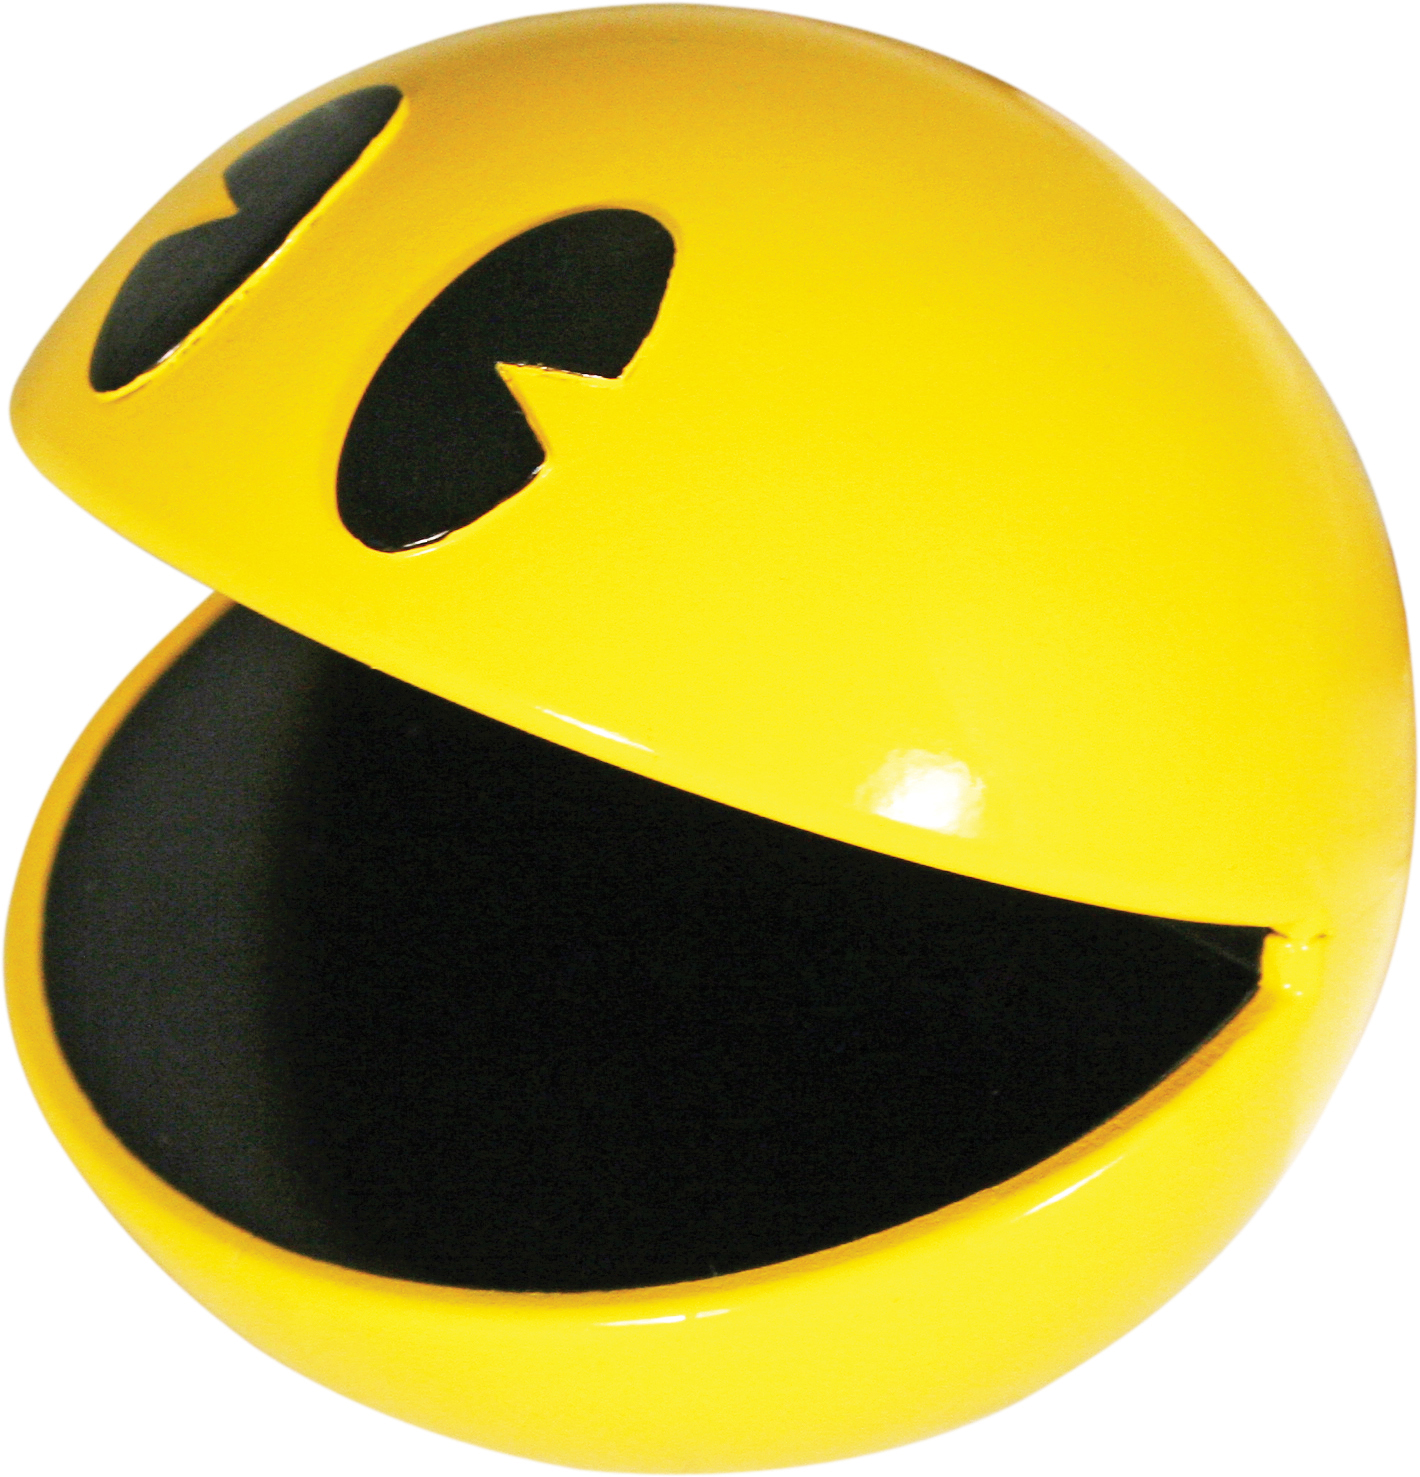
\includegraphics[width=0.5\linewidth]{Documentation/Images/Pacman.jpg}
	\end{minipage}
	\hfill
	\begin{minipage}{0.45\textwidth}
		\centering
		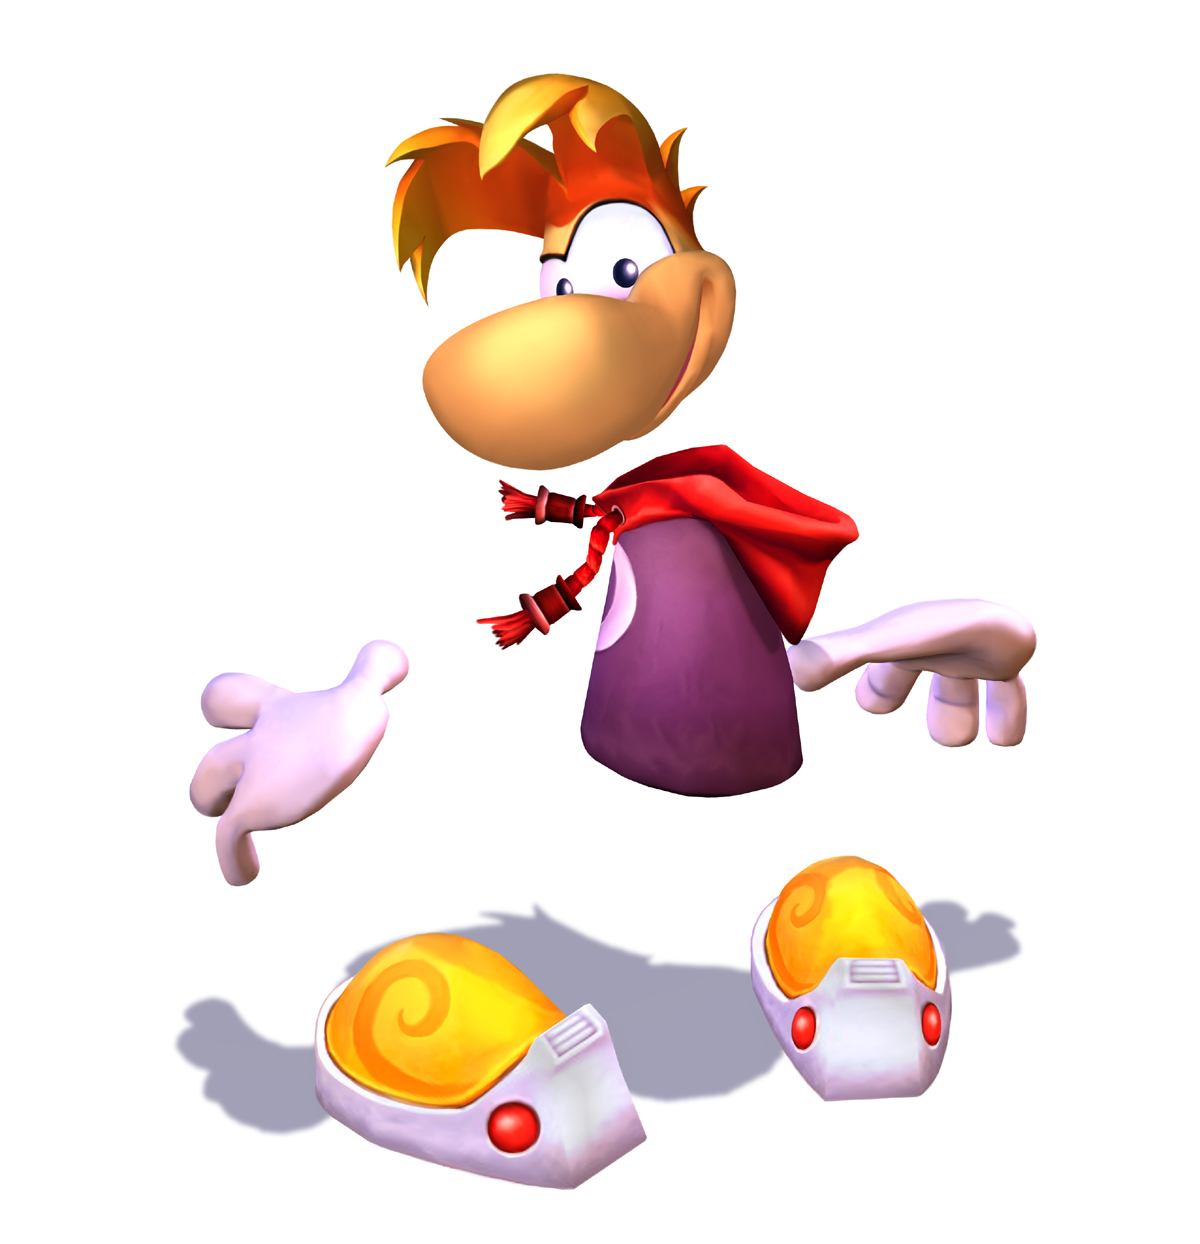
\includegraphics[width=0.5\linewidth]{Documentation/Images/Rayman.jpg}
	\end{minipage}
	\caption{\textit{Links:} Der Pacman, der die Grundlage für die Minimon-Figur darstellt. \textit{Rechts:} Der Rayman, bei dem die Arme und Beine praktisch in der Luft schweben.}
	\label{fig:character_design}
\end{figure}

Das Ziel beim Entwerfen der Figur war, dass sie kinderfreundlich sein sollte. Gleichzeitig soll sie auf den Betrachter leicht gruselig und bedrohlich (schließlich greifen sie die Erde an) wirken. Aus diesem Grund haben wir uns für einen weit aufgerissenen Mund entschieden. 

\begin{comment}
	\url{http://www.rayman-fanpage.de/rayman3_neu/grafik_rayman/rayman_1200.jpg}
	
	\url{http://www.truffleshuffle.co.uk/store/images_high_res/Pac_Man_Bottle_Opener_hi_res.jpg}
\end{comment}
